\documentclass[aspectratio=169]{../latex_main/tntbeamer}  % you can pass all options of the beamer class, e.g., 'handout' or 'aspectratio=43'
\usepackage{dsfont}
\usepackage{bm}
\usepackage[english]{babel}
\usepackage[T1]{fontenc}
%\usepackage[utf8]{inputenc}
\usepackage{graphicx}
\graphicspath{ {./figures/} }
\usepackage{algorithm}
\usepackage[ruled,vlined,algo2e,linesnumbered]{algorithm2e}
\usepackage{hyperref}
\usepackage{booktabs}
\usepackage{mathtools}

\usepackage{amsmath,amssymb}

\DeclareMathOperator*{\argmax}{arg\,max}
\DeclareMathOperator*{\argmin}{arg\,min}

\usepackage{amsbsy}
\newcommand{\vect}[1]{\bm{#1}}
%\newcommand{\vect}[1]{\boldsymbol{#1}}

\usepackage{pgfplots}
\pgfplotsset{compat=1.16}
\usepackage{tikz}
\usetikzlibrary{trees} 
\usetikzlibrary{shapes.geometric}
\usetikzlibrary{positioning,shapes,shadows,arrows,calc,mindmap}
\usetikzlibrary{positioning,fadings,through}
\usetikzlibrary{decorations.pathreplacing}
\usetikzlibrary{intersections}
\pgfdeclarelayer{background}
\pgfdeclarelayer{foreground}
\pgfsetlayers{background,main,foreground}
\tikzstyle{activity}=[rectangle, draw=black, rounded corners, text centered, text width=8em]
\tikzstyle{data}=[rectangle, draw=black, text centered, text width=8em]
\tikzstyle{myarrow}=[->, thick, draw=black]

% Define the layers to draw the diagram
\pgfdeclarelayer{background}
\pgfdeclarelayer{foreground}
\pgfsetlayers{background,main,foreground}

% Requires XeLaTeX or LuaLaTeX
%\usepackage{unicode-math}

\usepackage{fontspec}
%\setsansfont{Arial}
\setsansfont{RotisSansSerifStd}[ 
Path=../latex_main/fonts/,
Extension = .otf,
UprightFont = *-Regular,  % or *-Light
BoldFont = *-ExtraBold,  % or *-Bold
ItalicFont = *-Italic
]
\setmonofont{Cascadia Mono}[
Scale=0.8
]

% scale factor adapted; mathrm font added (Benjamin Spitschan @TNT, 2021-06-01)
%\setmathfont[Scale=1.05]{Libertinus Math}
%\setmathrm[Scale=1.05]{Libertinus Math}

% other available math fonts are (not exhaustive)
% Latin Modern Math
% XITS Math
% Libertinus Math
% Asana Math
% Fira Math
% TeX Gyre Pagella Math
% TeX Gyre Bonum Math
% TeX Gyre Schola Math
% TeX Gyre Termes Math

% Literature References
\newcommand{\lit}[2]{\href{#2}{\footnotesize\color{black!60}[#1]}}

%%% Beamer Customization
%----------------------------------------------------------------------
% (Don't) Show sections in frame header. Options: 'sections', 'sections light', empty
\setbeamertemplate{headline}{empty}

% Add header logo for normal frames
\setheaderimage{
	% 
\includegraphics[height=\logoheight]{figures/TNT_darkv4.pdf}
	
\includegraphics[height=\logoheight]{../latex_main/figures/luh_logo_rgb_0_80_155.pdf}
	% 
\includegraphics[height=\logoheight]{figures/logo_tntluh.pdf}
}

% Header logo for title page
\settitleheaderimage{
	% 
\includegraphics[height=\logoheight]{figures/TNT_darkv4.pdf}
	
\includegraphics[height=\logoheight]{../latex_main/figures/luh_logo_rgb_0_80_155.pdf}
	% 
\includegraphics[height=\logoheight]{figures/logo_tntluh.pdf}
}

% Title page: tntdefault 
\setbeamertemplate{title page}[tntdefault]  % or luhstyle
% Add optional title image here
%\addtitlepageimagedefault{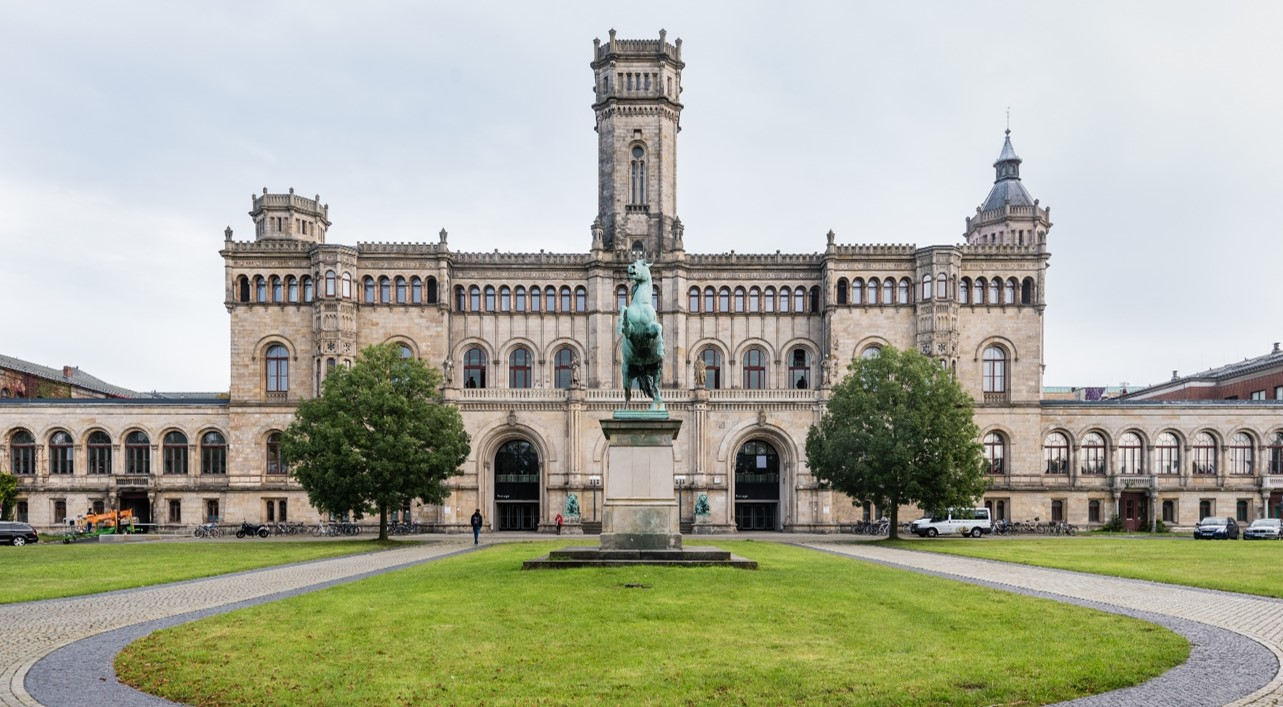
\includegraphics[width=0.65\textwidth]{figures/luh_default_presentation_title_image.jpg}}

% Title page: luhstyle
% \setbeamertemplate{title page}[luhstyle]
% % Add optional title image here
% \addtitlepageimage{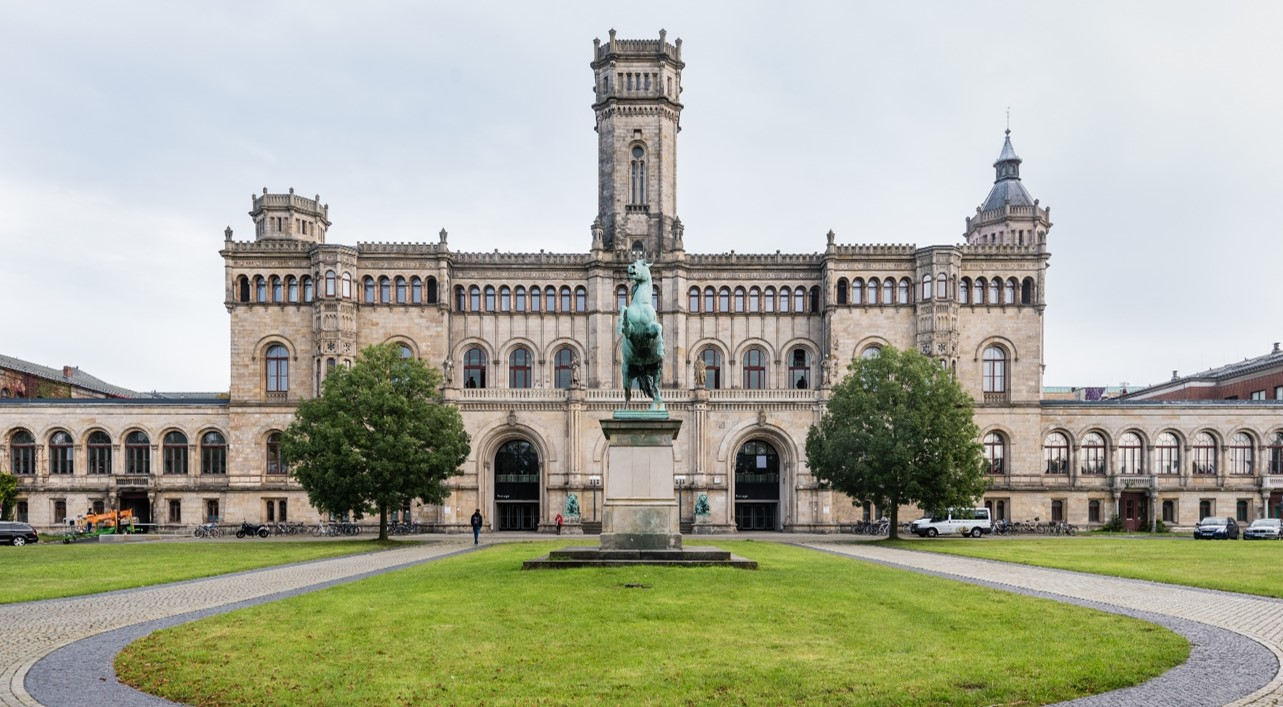
\includegraphics[width=0.75\textwidth]{figures/luh_default_presentation_title_image.jpg}}

\author[Abedjan \& Lindauer]{Ziawasch Abedjan \& Marius Lindauer\\[1em]
	
\includegraphics[height=\logoheight]{../latex_main/figures/luh_logo_rgb_0_80_155.pdf}\qquad
	
\includegraphics[height=\logoheight]{../latex_main/figures/DBIS_Kurzlogo.png}\qquad

\includegraphics[height=\logoheight]{../latex_main/figures/TNT_darkv4}\qquad

\includegraphics[height=\logoheight]{../latex_main/figures/L3S.jpg}	}
\date{Summer Term 2022; \hspace{0.5em} {
\includegraphics[height=1.5em]{../latex_main/figures/Cc-by-nc-sa_icon.svg.png}}; based on \href{https://ds100.org/fa21/}{[DS100]}
}


%%% Custom Packages
%----------------------------------------------------------------------
% Create dummy content
\usepackage{blindtext}

% Adds a frame with the current page layout. Just call \layout inside of a frame.
\usepackage{layout}


%%% Macros
%\renewcommand{\vec}[1]{\mathbf{#1}}
% \usepackage{bm}
%\let\vecb\bm

\title[LR: Derivation]{DS: Classification}
\subtitle{Deriving Logistic Regression}

\graphicspath{ {./figure/} }
%\institute{}


\begin{document}
	
	\maketitle
	\begin{frame}{Example dataset}
	    \begin{columns}
	        \begin{column}{.4\textwidth}
	                In this lecture, we will primarily use data from the 2017-18 NBA season.\\  \bigskip
	                Goal: Predict whether or not a team will win, given their FG\_PCT\_DIFF.
	                \begin{itemize}
	                    \item This is the difference in field goal percentage between the two teams.
	                    \item Positive FG\_PCT\_DIFF: team made more shots than the opposing team.
	                \end{itemize}
	        \end{column}
	        
	        \begin{column}{.4\textwidth}

	                    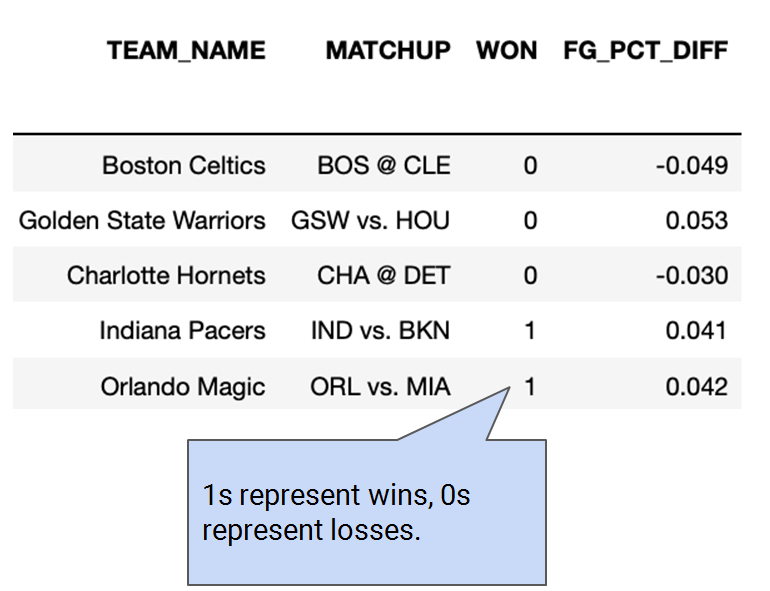
\includegraphics[scale=.35]{Bild3}
	                    
	        \end{column}
	    \end{columns}
	\end{frame}
	
	
	\begin{frame}{Why not use Ordinary Least Squares?}
	    \begin{columns}
	        \begin{column}{.4\textwidth}
	                We already have a model that can predict any quantitative response. Why not use it here?
	                \begin{itemize}
	                    \item The output can be outside of the range [0, 1]. What does a predicted WON value of -2 mean?
	                    \item Very sensitive to outliers.
	                    \item Many other statistical reasons.
	                    \begin{itemize}
	                        \item Not the point of our class.
	                    \end{itemize}
	                \end{itemize}
	        \end{column}
	        
	        \begin{column}{.4\textwidth}

	                    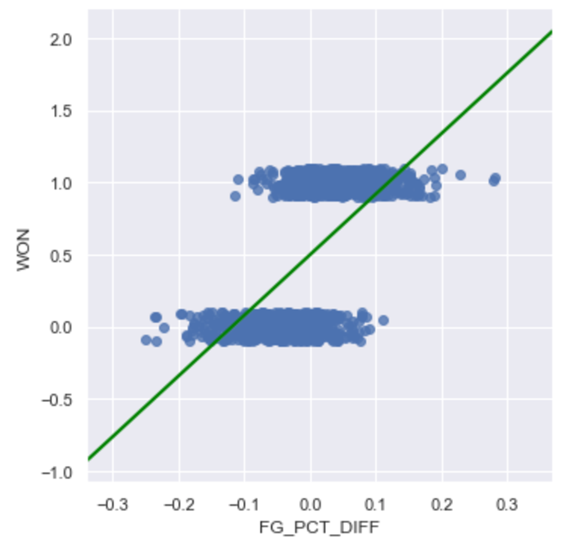
\includegraphics[scale=.5]{Bild4}
	        \end{column}
	    \end{columns}
	\end{frame}
	
	
		\begin{frame}{Graph of averages}
	    \begin{columns}
	        \begin{column}{.5\textwidth}
	                When defining the simple linear regression model, we binned the x-axis, and took the average y-value for each bin, and tried to model that.\\
	                \bigskip
	                Doing so here yields a curve that resembles an s.
	                \begin{itemize}
	                    \item Since our true y is either 0 or 1, this curve models the probability that WON = 1, given FG\_PCT\_DIFF.
	                    \begin{itemize}
	                        \item WON = 1 means “belong to class 1”.
	                    \end{itemize}
	                    \item Our goal is to model this red curve as best as possible.
	                \end{itemize}
	        \end{column}
	        
	        \begin{column}{.4\textwidth}

	                    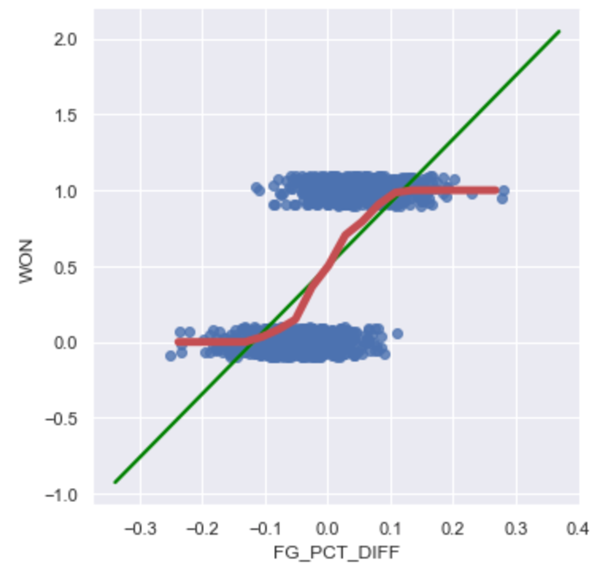
\includegraphics[scale=.5]{Bild5}
	        \end{column}
	    \end{columns}
	\end{frame}
	
	
	\begin{frame}{Log-odds of probability is roughly linear}
	    The log-odds of the probability of belonging to Class 1 ($p = 1$) was linear. This is the assumption that logistic regression is based on. \\
	    \begin{equation*}
	        \text{odds(p)} = \frac{p}{1 - p}\hspace{1cm} \text{log-odds(p)} = \text{log}\left(\frac{p}{1 - p}\right)
	    \end{equation*}
	    
	    For now, let’s denote $t$ as our linear function (since log-odds is linear). Solving for p:
	    \begin{align*}
	        t &= \text{log}\left(\frac{p}{1 - p}\right)\rightarrow \text{With logistic regression, we are always referring to log base e (“ln”).
} \\
	        e^t &= \frac{p}{1 - p}\\
	        e^t - pe^t &= p\\
	        p &= \frac{e^t}{1 + e^t} = \frac{1}{1 + e^{-t}}
	    \end{align*}
	\end{frame}
	
	\begin{frame}{Log-odds of probability is roughly linear}
	    The log-odds of the probability of belonging to class 1 was linear. This is the assumption that logistic regression is based on. \\
	    \begin{equation*}
	        \text{odds(p)} = \frac{p}{1 - p}\hspace{1cm} \text{log-odds(p)} = \text{log}\left(\frac{p}{1 - p}\right)
	    \end{equation*}
	    
	    For now, let’s let t denote our linear function (since log-odds is linear). Solving for p:
	    \begin{align*}
	        t &= \text{log}\left(\frac{p}{1 - p}\right)\\
	        e^t &= \frac{p}{1 - p}\\
	        e^t - pe^t &= p\\
	    \end{align*}
	\end{frame}
	
	
	
	\begin{frame}{Arriving at the logistic regression model}
	    We know how to model linear functions quite well.\\
	    \begin{itemize}
	        \item We can substitute          $t = \bm{x}^\intercal\bm{\theta} $           , since t was just a placeholder.
	    \end{itemize}
	    \begin{equation*}
	        p = \frac{1}{1 + e^{-t}} = \sigma (t)
	    \end{equation*}
	    p represents the probability of belonging to class 1.
	    \begin{itemize}
	        \item We are modeling          $P(Y=1|\bm{x})$.
	    \end{itemize}
	    Putting this all together:
	    \begin{equation*}
	        P(Y=1|\bm{x}) = \frac{1}{1 + e^{-\bm{x}^\intercal\bm{\theta}}} = \sigma(\bm{x}^\intercal\bm{\theta})
	    \end{equation*}
	    Looks just like the linear regression model, with a $\sigma()$ wrapped around it.
We call logistic regression a generalized linear model, since it is a non-linear transformation of a linear model.

	\end{frame}
	
	\begin{frame}{Arriving at the logistic regression model}
	    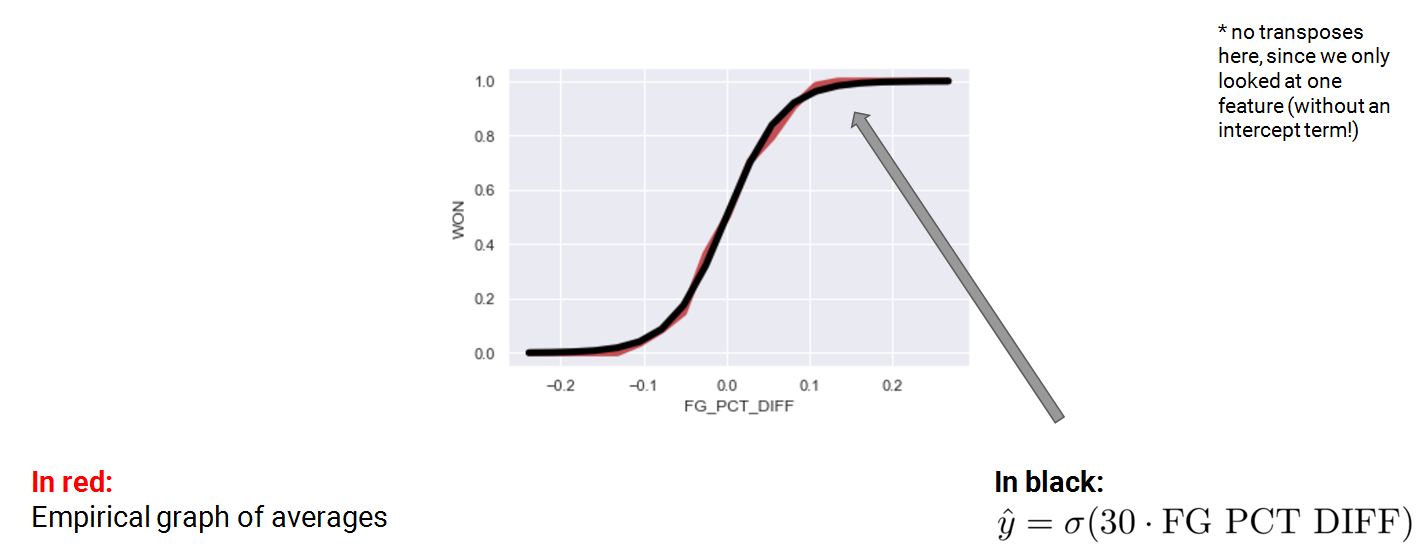
\includegraphics[scale=.4]{Bild6}
	\end{frame}
	
	\begin{frame}{Shape of the logistic function}
	   
	   \begin{columns}
	    
	   \begin{column}{.4\textwidth}
	   Consider the plot of       $\sigma (\bm{x}^\intercal\bm{\theta_1})$      , for several different values of $\bm\theta_1$. 
	   \begin{itemize}
	       \item If $\bm\theta_1$ is positive, the curve increases to the right.
	       \item The further  $\bm\theta_1$ is from 0, the steeper the curve.
	   \end{itemize}
	   \end{column}
	    
	    \begin{column}{.6\textwidth}

	            \centering	            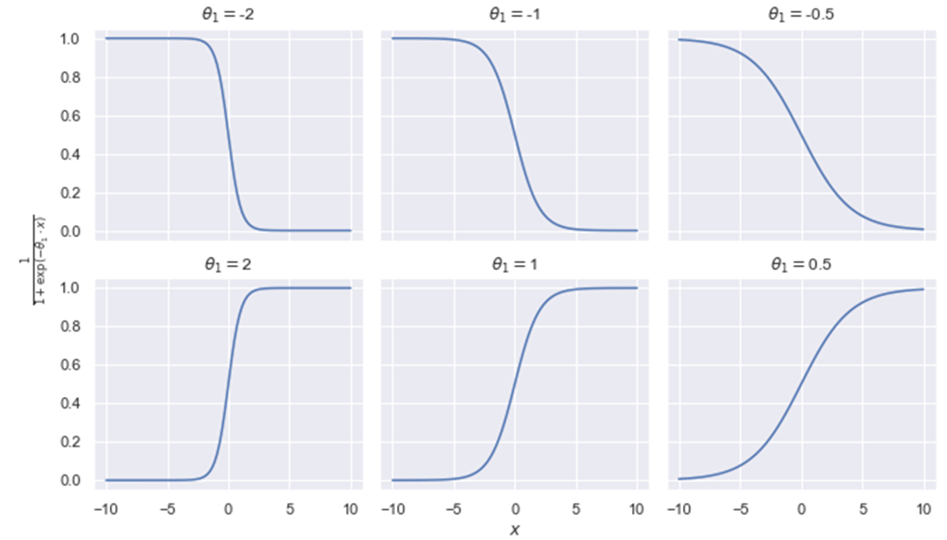
\includegraphics[width=\textwidth]{Bild10}
	            
	    \end{column}
	    
	    \end{columns}
	\end{frame}
	
\end{document}